\documentclass{article}
\usepackage{amsmath,amsthm,amssymb,amsfonts}
\usepackage{setspace,enumitem}
\usepackage{graphicx}
\usepackage{hyperref}
\usepackage{natbib}
\usepackage{afterpage}
\usepackage{xcolor}
\usepackage{etoolbox}
\usepackage{booktabs}
\usepackage{pdfpages}
\usepackage{multicol}
\usepackage{geometry}
\usepackage{accents}
\usepackage{bbm}
\usepackage{placeins}
\usepackage{verbatim}
\hypersetup{
	colorlinks,
	linkcolor={blue!90!black},
	citecolor={red!90!black},
	urlcolor={blue!90!black}
}

\newtheorem{theorem}{Theorem}
\newtheorem{assumption}{Assumption}
\newtheorem{definition}{Definition}
\newtheorem{lemma}{Lemma}
\setlength{\parindent}{0cm}
\geometry{margin = 1in}

\newcommand{\R}{\mathbb{R}}
\newcommand{\ubar}[1]{\underaccent{\bar}{#1}}
\newcommand{\Int}{\text{Int}}
\newcommand{\xbf}{\mathbf{x}}
\newcommand{\Abf}{\mathbf{A}}
\newcommand{\Bbf}{\mathbf{B}}
\newcommand{\Gbf}{\mathbf{G}}
\newcommand{\bbf}{\mathbf{b}}
\newcommand{\one}{\mathbbm{1}}

\newtoggle{extended}
\settoggle{extended}{false}

\title{FIN 970: Homework 1}
\author{Alex von Hafften }

\begin{document}

\maketitle


\section{Problem 1: GMM Estimation of a Linear Regression Model}

Write a code to implement a GMM estimation of a linear regression model, $Y_t = \beta'X_t + u_t$. The code should produce the point estimates and the Newey-West standard errors of $\beta$ and the regression $R^2$. We will use this code in later assignments to evaluate statistical significance of predictability evidence

\bigskip

\textbf{Solution:} See \texttt{gmm.jl} for implementation (also in appendix). Also see \texttt{gmm\_test.jl} for a test of the GMM estimation using simulated data (also in appendix).

\section{Problem 2: Bayesian Estimation of an Autoregressive Model}

Consider an $AR(1)$ model for $y^T = \{y_t\}_{t=1}^T$:

$$
y_{t+1} = \mu + \rho y_t+ \sigma \varepsilon_{t+1}
$$

where $\varepsilon \sim_{iid} N(0, 1)$

\begin{enumerate}

\item Consider independent conjugate priors for the model parameters,

$$
\mu \sim N(m, s^2), \rho \sim N(\tilde\rho, \omega^2), \sigma^2 \sim IG(\alpha/2, \beta/2)
$$

Show that the conditional posteriors are given by

$$
\mu | y^T, \rho, \sigma \sim N, \rho | y^T, \mu, \sigma \sim N, \sigma^2 | y^T, \mu, \rho \sim IG
$$

Find the parameters of the posterior distributions in terms of the parameters of the prior and
the data.

\textbf{Solution:} The priors for the model parameters imply:

\begin{align*}
\mu &\sim N(m, s^2)\\
\implies f(\mu) 
&= \frac{1}{\sqrt{2\pi s^2}} \exp \Bigg( - \frac{1}{2s^2} (\mu - m)^2\Bigg) 
\propto \exp \Bigg( - \frac{1}{2s^2} (\mu^2 - 2\mu m) \Bigg) \\
\rho &\sim N(\tilde\rho, \omega^2) \\
\implies f(\rho) 
&= \frac{1}{\sqrt{2\pi \omega^2}} \exp \Bigg( - \frac{1}{2 \omega^2} (\rho - \tilde\rho)^2\Bigg) 
\propto \exp \Bigg( - \frac{1}{2\omega^2} (\rho^2 - 2\rho \tilde \rho) \Bigg) \\ 
\sigma^2 &\sim IG(\alpha/2, \beta/2) \\
\implies f(\sigma^2)
&= \frac{(\beta/2)^{(\alpha/2)}}{\Gamma(\alpha/2)} (\sigma^2)^{-\alpha/2 - 1} \exp\Bigg( - \frac{\beta}{2\sigma^2} \Bigg)  
\propto \sigma^{2(-\alpha/2 - 1)} \exp \Bigg( - \frac{\beta}{2\sigma^2}\Bigg)
\end{align*}

From the $AR(1)$ structure, we know that 

\begin{align*}
y_{t} | \mu, \rho, \sigma, y_{t-1} &\sim N(\mu + \rho y_{t-1}, \sigma^2) \\ 
f(y_t|y_{t-1}, \mu, \rho, \sigma) &= \frac{1}{\sqrt{2\pi \sigma^2}} \exp \Bigg( - \frac{1}{2 \sigma^2} (y_t - \mu - \rho y_{t-1})^2\Bigg) \\
&= \frac{1}{\sqrt{2\pi \sigma^2}} \exp \Bigg( - \frac{1}{2 \sigma^2} (y_t^2 + \mu^2 + \rho^2 y_{t-1}^2 - 2\mu y_t - 2 \rho y_{t-1}y_t + 2\rho \mu y_{t-1})\Bigg) \\
&\propto \frac{1}{\sigma}\exp \Bigg( - \frac{1}{2 \sigma^2} (y_t^2 + \mu^2 + \rho^2 y_{t-1}^2 - 2\mu y_t - 2 \rho y_{t-1}y_t + 2\rho \mu y_{t-1})\Bigg)
\end{align*}

Furthermore, assuming $y_0$ is given (so $f(y_0|\mu, \rho, \sigma) = 1$):

\begin{align*}
f(y^T|\mu, \rho, \sigma) 
&= f(y_T|\mu, \rho, \sigma, y_{T-1}) \cdot ... \cdot f(y_1|\mu, \rho, \sigma, y_0) f(y_0|\mu, \rho, \sigma) \\
&= \prod_{t=1}^T f(y_t |\mu, \rho, \sigma, y_{t-1})\\
&\propto \prod_{t=1}^T \frac{1}{\sigma}\exp \Bigg( - \frac{1}{2 \sigma^2} (y_t^2 + \mu^2+ \rho^2 y_{t-1}^2 - 2\mu y_t - 2 \rho y_{t-1}y_t + 2\rho \mu y_{t-1})\Bigg)\\
&= \frac{1}{\sigma^T} \exp \Bigg(\sum_{t=1}^T  - \frac{1}{2 \sigma^2} (y_t^2 + \mu^2+ \rho^2 y_{t-1}^2 - 2\mu y_t - 2 \rho y_{t-1}y_t + 2\rho \mu y_{t-1})\Bigg)\\
&= \frac{1}{\sigma^T} \exp \Bigg( - \frac{1}{2 \sigma^2} (\sum_{t=1}^T y_t^2 + T\mu^2 + \rho^2 \sum_{t=1}^T y_{t-1}^2 - 2\mu \sum_{t=1}^T y_t - 2 \rho \sum_{t=1}^T y_{t-1}y_t + 2\rho \mu \sum_{t=1}^T y_{t-1})\Bigg)\\
&= \frac{1}{\sigma^T} \exp \Bigg( - \frac{T}{2 \sigma^2} (\overline{y_T^2} + \mu^2 +  \rho^2 \overline{y_{T-1}^2} - 2\mu \overline{ y_T } - 2 \rho \overline{ z_T} + 2\rho \mu \overline{y_{T-1}})\Bigg)
\end{align*}

where

\begin{align*}
\overline{y_{T}^2} &\equiv \frac{1}{T} \sum_{t=1}^{T} y_t^2\\
\overline{y_{T-1}^2} &\equiv \frac{1}{T} \sum_{t=1}^{T} y_{t-1}^2\\
\overline{y_{T}} &\equiv \frac{1}{T} \sum_{t=1}^{T} y_{t}\\
\overline{y_{T-1}} &\equiv \frac{1}{T} \sum_{t=1}^{T} y_{t-1}\\
\overline{z_{T}} &\equiv \frac{1}{T} \sum_{t=1}^{T} y_ty_{t-1}\\
\end{align*}

\pagebreak

Applying Bayes' Rule for $\mu$, we know that:

\begin{align*}
f(\mu|y^T, \rho, \sigma) &\propto f(\mu) f(y^T|\mu, \rho, \sigma)\\
&\propto \frac{1}{\sigma^T} \exp \Bigg( - \frac{1}{2s^2} (\mu^2 - 2\mu m) \Bigg) \exp \Bigg( - \frac{T}{2 \sigma^2} (\overline{y_T^2} + \mu^2  + \rho^2 \overline{y_{T-1}^2} - 2\mu \overline{ y_T } - 2 \rho \overline{ z_T} + 2\rho \mu \overline{y_{T-1}})\Bigg)\\
&\propto \exp \Bigg( - \frac{1}{2s^2} (\mu^2 - 2\mu m) \Bigg) \exp \Bigg( - \frac{T}{2 \sigma^2} (\mu^2  + 2\rho \mu \overline{y_{T-1}}- 2\mu \overline{ y_T })\Bigg)\\
&= \exp \Bigg( - \frac{1}{2s^2} (\mu^2 - 2\mu m) - \frac{T}{2 \sigma^2} (\mu^2  + 2\rho \mu \overline{y_{T-1}}- 2\mu \overline{ y_T })\Bigg)\\
&= \exp \Bigg(- \frac{1}{2}\Bigg(\mu^2\Bigg(\frac{1}{s^2} + \frac{T}{\sigma^2} \Bigg) - 2\mu \Bigg(\frac{m}{2s^2} + \frac{T(\rho  \overline{y_{T-1}}- \overline{ y_T }))}{2 \sigma^2} \Bigg)\Bigg)\Bigg)\\
&= \exp \Bigg(- \frac{1}{2\Big(\frac{1}{s^2} + \frac{T}{\sigma^2} \Big)^{-1}}\Bigg(\mu^2 - 2\mu \Bigg(\frac{m}{2s^2} + \frac{T(\rho  \overline{y_{T-1}}- \overline{ y_T }))}{2 \sigma^2} \Bigg)\Bigg(\frac{1}{s^2} + \frac{T}{\sigma^2} \Bigg)^{-1}\Bigg)\Bigg)
\end{align*}

Thus, $\mu| y^T, \mu, \rho, \sigma \sim N(\tilde{m}, \tilde{s}^2)$ where $\nu_\mu\equiv \frac{\sigma^2}{s^2}$ and:

\begin{align*}
\tilde{s}^2 
&\equiv \Bigg(\frac{1}{s^2} + \frac{T}{\sigma^2} \Bigg)^{-1} \\
&= \Bigg(\frac{\nu_\mu}{\sigma^2} + \frac{T}{\sigma^2} \Bigg)^{-1} \\
&= \frac{\sigma^2}{\nu_\mu+T} \\
\tilde{m} 
&\equiv \Bigg(\frac{m}{2s^2} + \frac{T(\rho  \overline{y_{T-1}}- \overline{ y_T }))}{2 \sigma^2} \Bigg)\Bigg(\frac{1}{s^2} + \frac{T}{\sigma^2} \Bigg)^{-1}\\
&= \Bigg(\frac{m\nu_\mu + T(\rho  \overline{y_{T-1}}- \overline{ y_T }))}{2 \sigma^2} \Bigg) \frac{\sigma^2}{\nu_\mu+T}\\
&= m \frac{\nu_\mu}{\nu_\mu + T} + (\rho  \overline{y_{T-1}}- \overline{ y_T })\frac{T}{\nu_\mu + t}
\end{align*}

\pagebreak

Applying Bayes' Rule for $\rho$, we know that:

\begin{align*}
f(\rho|y^T, \sigma, \mu) &\propto f(\rho) f(y^T|\mu, \rho, \sigma)\\
&\propto \frac{1}{\sigma^T} \exp \Bigg( - \frac{1}{2\omega^2} (\rho^2 - 2\rho \tilde \rho) \Bigg) \exp \Bigg( - \frac{T}{2 \sigma^2} (\overline{y_T^2} + \mu^2  + \rho^2 \overline{y_{T-1}^2} - 2\mu \overline{ y_T } - 2 \rho \overline{ z_T} + 2\rho \mu \overline{y_{T-1}})\Bigg)\\
&\propto \exp \Bigg( - \frac{1}{2\omega^2} (\rho^2 - 2\rho \tilde \rho) - \frac{T}{2 \sigma^2} (\rho^2 \overline{y_{T-1}^2} - 2 \rho \overline{ z_T} + 2\rho \mu \overline{y_{T-1}})\Bigg) \\
&= \exp \Bigg(-\frac{1}{2}  \Bigg(\rho^2 \Bigg(\frac{1}{\omega^2} + \frac{T\overline{y_{T-1}^2}}{\sigma^2}\Bigg)  +  2\rho\Bigg( \frac{\tilde\rho}{\omega^2} + \frac{T\overline{ z_T}}{\sigma^2} - \frac{T\mu\overline{y_{T-1}}}{\sigma^2} \Bigg)\Bigg)\Bigg)\\
&= \exp \Bigg(-\frac{1}{2\Big(\frac{1}{\omega^2} + \frac{T\overline{y_{T-1}^2}}{\sigma^2}\Big)^{-1}}  \Bigg(\rho^2   +  2\rho\Bigg( \frac{\tilde\rho}{\omega^2} + \frac{T\overline{ z_T}}{\sigma^2} - \frac{T\mu\overline{y_{T-1}}}{\sigma^2} \Bigg)\Bigg(\frac{1}{\omega^2} + \frac{T\overline{y_{T-1}^2}}{\sigma^2}\Bigg)^{-1}\Bigg)\Bigg)
\end{align*}

Thus, $\rho | y^T, \mu, \rho, \sigma \sim N(\tilde{\tilde{\rho}}, \tilde{\omega}^2)$ where $\nu_\rho\equiv \frac{\sigma^2}{\omega^2}$ and:

\begin{align*}
\tilde{\omega}^2
&\equiv \Bigg(\frac{1}{\omega^2} + \frac{T\overline{y_{T-1}^2}}{\sigma^2}\Bigg)^{-1}\\
&= \Bigg(\frac{\nu_\rho}{\sigma^2} + \frac{T\overline{y_{T-1}^2}}{\sigma^2}\Bigg)^{-1}\\
&= \frac{\sigma^2}{\nu_\rho + T\overline{y_{T-1}^2}}\\
\tilde{\tilde{\rho}}
&= \Bigg( \frac{\tilde\rho\nu_\rho}{\sigma^2} + \frac{T\overline{ z_T}}{\sigma^2} - \frac{T\mu\overline{y_{T-1}}}{\sigma^2} \Bigg)  \frac{\sigma^2}{\nu_\rho + T\overline{y_{T-1}^2}}\\
&=  \frac{\nu_\rho}{\nu_\rho + T\overline{y_{T-1}^2}}\tilde\rho + \frac{T}{\nu_\rho + T\overline{y_{T-1}^2}} [\overline{ z_T} - \mu\overline{y_{T-1}}]
\end{align*}

Applying Bayes' Rule for $\sigma$, we know that:

\begin{align*}
f(\sigma|y^T, \rho, \mu) 
&\propto f(\rho) f(y^T|\mu, \rho, \sigma)\\
&\propto \frac{1}{\sigma^T} \sigma^{2(-\alpha/2 - 1)} \exp \Bigg( - \frac{\beta}{2\sigma^2}\Bigg) \exp \Bigg( - \frac{T}{2 \sigma^2} (\overline{y_T^2} + \mu^2 +  \rho^2 \overline{y_{T-1}^2} - 2\mu \overline{ y_T } - 2 \rho \overline{ z_T} + 2\rho \mu \overline{y_{T-1}})\Bigg)\\
&= \sigma^{2(-(\alpha+T)/2 - 1)} \exp \Bigg( - \frac{1}{2\sigma^2} [\beta + T (\overline{y_T^2} + \mu^2 +  \rho^2 \overline{y_{T-1}^2} - 2\mu \overline{ y_T } - 2 \rho \overline{ z_T} + 2\rho \mu \overline{y_{T-1}})]\Bigg)\\
\end{align*}

\pagebreak

Thus, $\sigma | y^T, \mu, \rho, \sigma \sim IG(\tilde{\alpha}/2, \tilde{\beta}/2)$ where:

\begin{align*}
\tilde{\alpha} &= \alpha + T\\
\tilde{\beta} &= \beta + T (\overline{y_T^2} + \mu^2 +  \rho^2 \overline{y_{T-1}^2} - 2\mu \overline{ y_T } - 2 \rho \overline{ z_T} + 2\rho \mu \overline{y_{T-1}})
\end{align*}


\item The Excel file \texttt{Longyielddata.xlsx} contains the annual data for long-term 10-year US
government bond yields from Global Financial Data (GFD) database. Choose the priors for the model parameters. For example, we can use fairly uninformative
priors:

\begin{center}
\begin{tabular}{ l | c c }
& Prior Mean & Prior Std. Dev. \\ 
\hline
 $\mu$  & 0.3 & 0.5  \\  
 $\rho$ & 0.95 & 0.2 \\
 $\sigma^2$ & 1 & 1
\end{tabular}
\end{center}

Design and implement an MCMC algorithm to draw a long sample from the joint posterior
distribution of the three parameters, where the sampling of each parameter is implemented
via Gibbs sampler.

\textbf{Solution:} See \texttt{gibbs.jl} for the implementation simulates a MCMC using a Gibbs sampler (also in appendix). See \texttt{gibbs\_run.jl} for code that runs a MCMC and plots the results (also in appendix). 

\item Run a long MCMC chain and discard appropriate number of initial draws due to burn-in.
Plot the three chains. Do the chains mix well? Does it look like they come from a stationary
distribution? How large is the persistence in the chains? Plot the autocorrelation plots for
the chains, and the scatter plots of each parameter against the others. You might find that
the most problematic is the persistence and cross-correlation between $\mu$ and $\rho$, and there's a good reason for it. Notice that $\mu$ is an intercept, and not the unconditional mean of $y_t$: $E(y) = \mu/(1 - \rho)$. So every time we change $\rho$, intuitively, the draw for $\mu$ has to adjust to
target the unconditional mean of the process. How would you change the problem to break
up this almost mechanical correlation between the parameters?

\textbf{Solution:} I simulate MCMC of length 1000 with a 100 periods for burn in.\footnote{Mean of inverse gamma distribution is $\beta/(\alpha-1)$ and variance is $\beta^2/((\alpha - 1)^2(\alpha-2))$. For unit mean and unit variance/standard deviation, $\alpha = 3$ and $\beta = 2$.}  The chains are plotted below:

\begin{center}

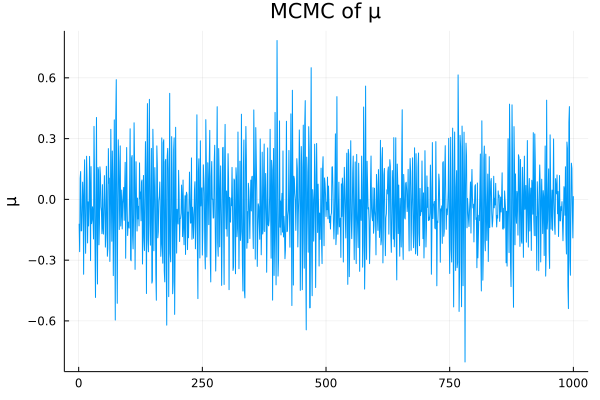
\includegraphics[scale=0.5]{p2_q3_mu.png}

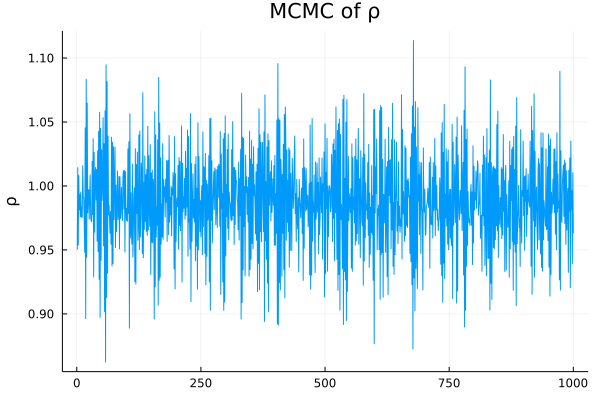
\includegraphics[scale=0.5]{p2_q3_rho.png}

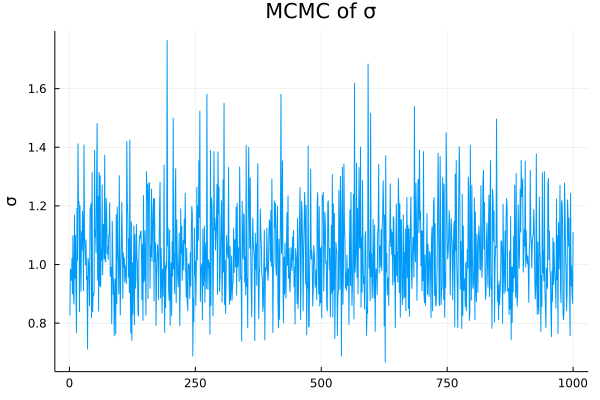
\includegraphics[scale=0.5]{p2_q3_sigma.png}

\end{center}

Yes, I think the chains mix pretty well. And yes, it looks like they come from a stationary distribution. The AR(1) coefficients for $\mu$ and $\rho$ are quite high in magnitude at around $-0.7$ while the AR(1) coefficient for $\sigma$ is relatively small in magnitude at around $-0.05$ (see below).  Thus, the persistence of $\sigma$ is low, but values $\mu$ and $\rho$ are typical succeeded by large values of the opposite sign.

\begin{center}
\begin{tabular}{ l | c c }
& Constant & Lagged Value \\ 
\hline
$\mu$  & -0.0442 & -0.7151 \\  
$\rho$ & 1.7036 & -0.7235  \\
$\sigma$ & 1.0792 & -0.0467
\end{tabular}
\end{center}

\pagebreak

The autocorrelation functions are plotted below. For $\mu$ and $\rho$, the autocorrelations bounce back and forth from negative to positive with diminishing magnitude, confirming the AR(1) coefficients.  For $\sigma$, the autocorrelation drops at the first lag is small for the rest of the lags.

\begin{center}

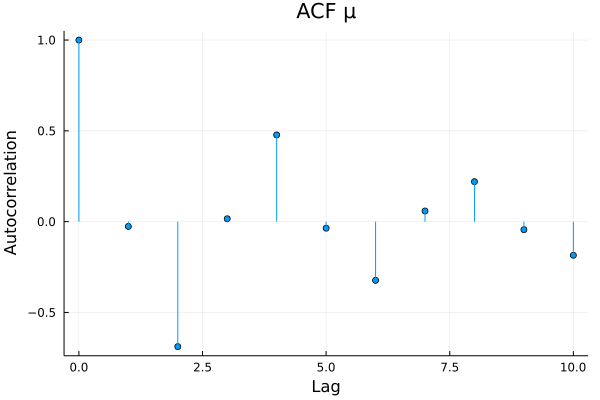
\includegraphics[scale=0.5]{p2_q3_mu_acf.png}

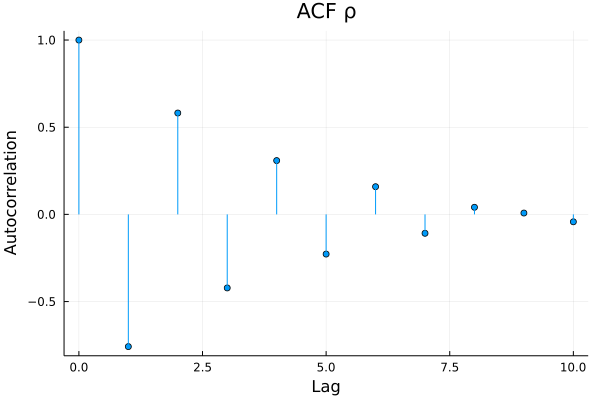
\includegraphics[scale=0.5]{p2_q3_rho_acf.png}

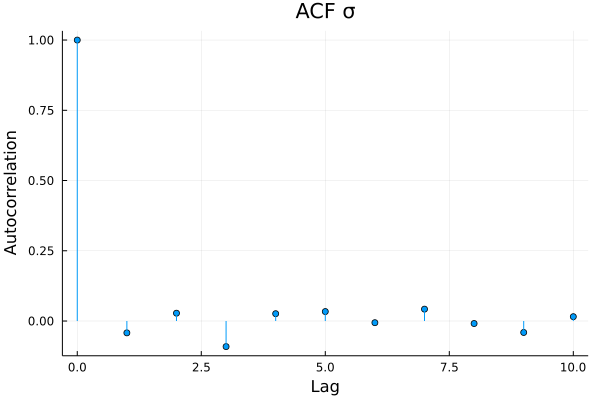
\includegraphics[scale=0.5]{p2_q3_sigma_acf.png}

\end{center}


The scatterplots of the simulated parameters are below.  These scatterplots confirm the analysis so far.  We see a similar pattern to the ACF plots when we look at $\mu$ relative to $\rho$. Since $\mu$ and $\rho$ are almost mechanically connected, there's a negative relationship. The scatterplots of $\rho$ and $\mu$ relative to $\sigma$ show basically a cloud of points.

\begin{center}

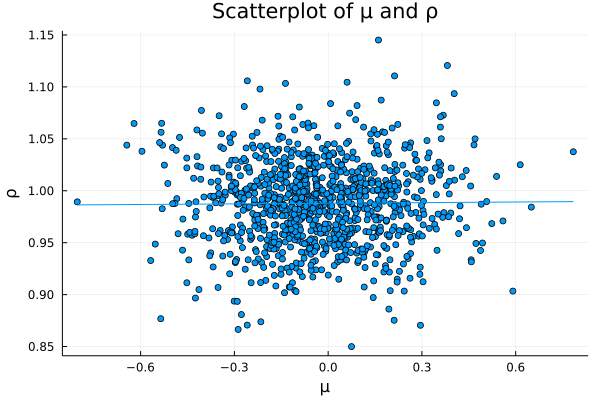
\includegraphics[scale=0.5]{p2_q3_mu_rho.png}

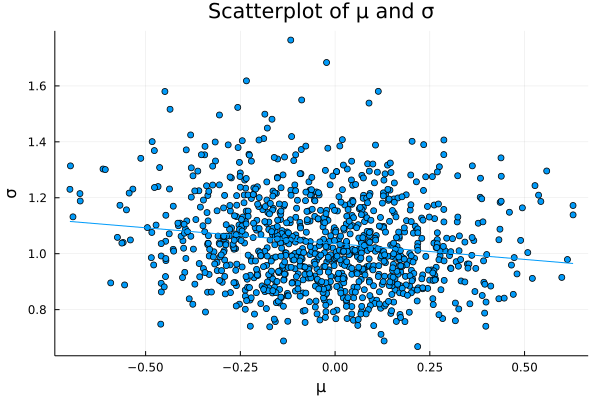
\includegraphics[scale=0.5]{p2_q3_mu_sigma.png}

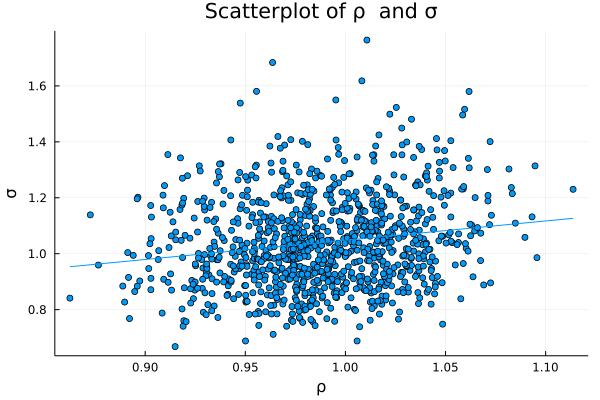
\includegraphics[scale=0.5]{p2_q3_rho_sigma.png}


\end{center}

We could fix this issue by simulating the chain and then only saving simulations every ten rounds where the ACF is basically zero.


\item Report the posterior means and standard deviations of the parameters - how different the
posterior means are from the prior, and from the standard OLS estimates in the data? How
do the prior and posterior standard deviations compare? Overall, do you think your results
look reasonable?

\begin{center}
\begin{tabular}{ l | c c c c}
& Prior Mean & Prior Std. Dev. & Post. Mean & Post. Std. Dev.  \\ 
\hline
 $\mu$  & 0.3 & 0.5 & -0.0267 & 0.2328 \\  
 $\rho$ & 0.95 & 0.2 & 0.9886 & 0.0412 \\
 $\sigma$ & 1 & 1 & 1.1186 & 0.2448
\end{tabular}
\end{center}

The posterior mean for $\mu$ is much different than the prior mean (-0.03 vs 0.3).  The posterior mean for $\rho$ is pretty close to the prior (0.99 vs 0.95).  The posterior mean for $\sigma$ is pretty close to the prior (1 vs 1.12).  The posterior standard deviation for all parameters is much small than the prior standard deviation.  That makes sense because we chose a relatively loose prior.  I'm suspicious of these results due to the strong correlation between draws as discussed in question 3.

\pagebreak

\item  If you carefully examine your chain for $\rho$, you might find that some draws are above 1. This
does not look reasonable, as we have good reasons to believe that interest rates are stationary.
Let's correct that. First, let's use a truncated Normal prior for $\rho$ to ensure that this parameter
is always in $(-1, 1)$:

$$
f(\rho) \propto N (\tilde\rho, \omega^2) \text{ if } \rho \in (-1, 1); f(\rho) = 0 \text{ otherwise}.
$$

Further, instead of using Gibbs to draw $\rho$, now let's use Independence Metropolis-Hastings
where the proposal density is equal to the Normal conditional posterior of $\rho$ you found in part 1. Design and implement the new MCMC algorithm. Notice that a new algorithm (known
as a Rejection Sampling) should be a very simple and intuitive modification of the previous
one.

\textbf{Solutions}  See \texttt{gibbs.jl} for implementation.  If the option \texttt{rho\_distribution} is set to \texttt{"truncated\_normal"}, then the normal distribution for $\rho$ is truncated to be between -1 and 1.  A resulting MCMC for $\rho$ looks like:

\begin{center}
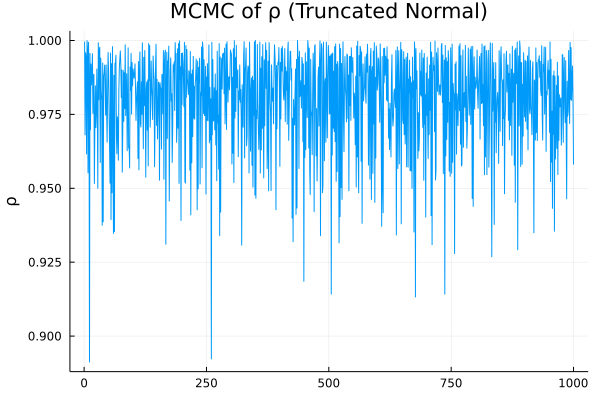
\includegraphics[scale =0.5]{p2_q5_rho_truncated_normal}
\end{center}

If the option \texttt{rho\_distribution} is set to \texttt{"imh"}, then Independence Metropolis-Hastings is used with the proposal density equal to the Normal conditional posterior of $\rho$. A resulting MCMC for $\rho$ looks like:

\begin{center}
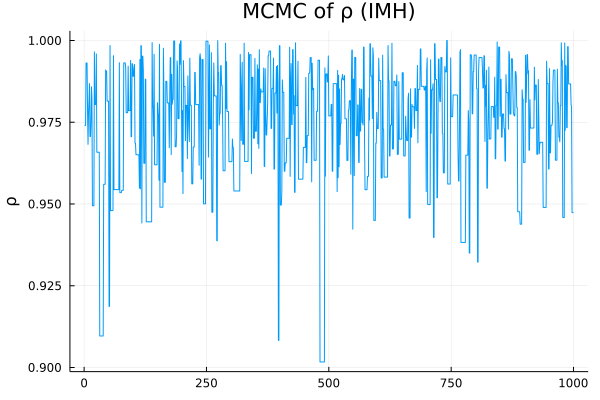
\includegraphics[scale =0.5]{p2_q5_rho_imh}
\end{center}


\item Examine the chain, report the posterior means and standard deviations. Overall, do you think your results look reasonable?

The posterior means and standard deviations across the three methods of simulating $\rho$ are below. Means and standard deviations for all parameters decrease compared to using normal sampling. For $\rho$, the means and standard deviations are lower with using a truncated normal and the MH.  This makes sense because we are limiting $\rho$ is be below one so the mean is lower.  It looks like $\rho$ is close to one though, so the simulations are generally closer to one, so the standard deviation is also lower.  This increase in $\rho$ reduces $\mu$ because of their ``almost" mechanical relationship with the unconditional mean.  It makes sense that if we're lower $\rho$, estimates of $\mu$ increase.  The standard deviation for $\mu$ also drops.

\begin{center}
\begin{tabular}{ l | c c c c c}
         &           & Prior & Normal  & Truncated Normal & MH  \\ 
\hline
$\mu$    & Mean      & 0.3   & -0.0267 & -0.0740 & -0.0981 \\  
         & Std. Dev. & 0.5   & 0.2328  & 0.1323 & 0.1437 \\  
$\rho$   & Mean      & 0.95  & 0.9886  & 0.9798 & 0.9726 \\
         & Std. Dev. & 0.2   & 0.0412  & 0.0161 & 0.0185 \\
$\sigma$ & Mean      & 1     & 1.1186  & 1.0481 & 1.0817 \\
         & Std. Dev. & 1     & 0.2448  & 0.1629 & 0.2007
\end{tabular}
\end{center}

Limiting $\rho \in [-1, 1]$, so seems to help to some degree with the strong relationship between $\mu$ and $\rho$, which we saw in the scatterplot of $\mu$ relative to $\rho$.

\begin{center}
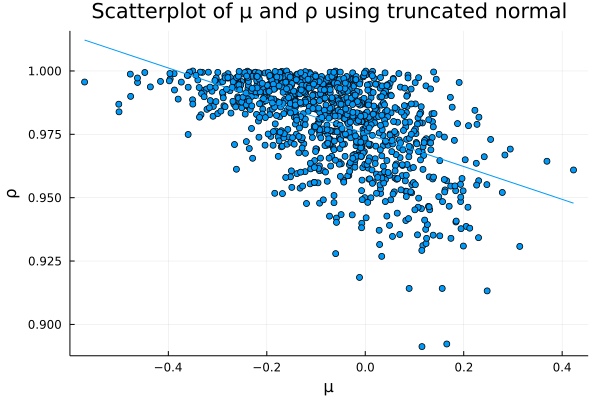
\includegraphics[scale =0.5]{p2_q6_mu_rho_truncated_normal}
\end{center}

\begin{center}
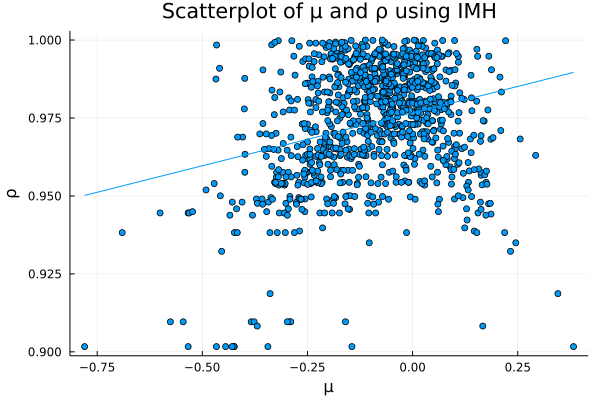
\includegraphics[scale =0.5]{p2_q6_mu_rho_imh}
\end{center}

\item Having simulation output from the MCMC chains makes it easy to compute, and assess
significance of, any complicated non-linear functions of the parameters and the data. Suppose
we are interested in $N = 5$ year forecast of yields from the model. Show that the forecast is
given by,

$$
E_ty_{t+N} = \mu \frac{1 - \rho^N}{1 - \rho} + \rho^N y_t
$$

Fix $t$. You can compute the implied forecast $(E_t y_{t+N})^i$ for each parameter draw from the chain $\theta^i$, for $i$ from 1 to $M$. Having the distribution of time-$t$ forecasts $\{(E_t y_{t+N})^i\}_{i=1}^M$, you
can numerically compute their mean, and 2.5\% - 97.5\% confidence band. Now do it for all $t$, and plot the posterior mean and the confidence band for the yield forecasts from the model.

\begin{center}
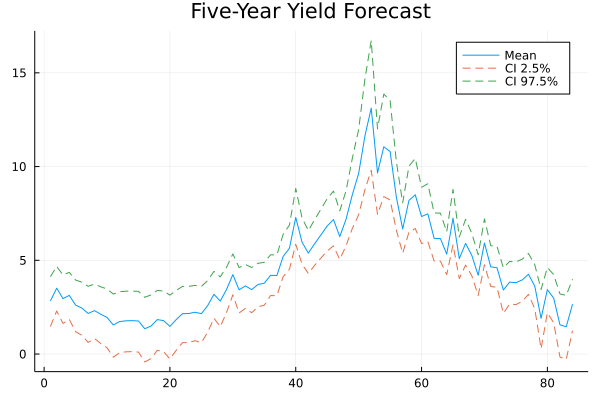
\includegraphics[scale =0.5]{p2_q6_forecast}
\end{center}

\end{enumerate}

\pagebreak

\section{Problem 3: Latent Drift Model}

Consider the following specification for consumption dynamics:

\begin{align*}
\Delta c_{t+1} &= \mu + x_t + \sigma_c \eta_{t+1},\\
x_{t+1} &= \rho x_t + \sigma_x e_{t+1},
\end{align*}

where $\eta$ and $e$ are independent (over time and from each other) shocks with mean zero and variance one.

\begin{enumerate}

\item We are interested in estimating the parameters of the model: $\mu, \sigma_c, \rho, \sigma_x$. Consider the following four moments: $E(\Delta c_t), Var(\Delta c_t), Cov(\Delta c_t, \Delta c_{t-1}), Cov(\Delta c_t, \Delta c_{t-2})$. Show that these four moments exactly identify the four unknown parameters. Describe how you would design and implement a GMM estimation of the model parameters based on these four moments. How would you infer the unobserved $x_t$ based on these estimates?

\bigskip

\textbf{Solutions:} We can rewrite $x_t$:

\begin{align*}
x_{t}
&= \rho x_{t-1} + \sigma_x e_{t} \\
&= \rho (\rho x_{t-2} + \sigma_x e_{t-1}) + \sigma_x e_{t} \\
&= \rho^2x_{t-2} + \sigma_x (\rho e_{t-1} + e_t)\\
&= \rho^2(\rho x_{t-3} + \sigma_x e_{t-2}) + \sigma_x (\rho e_{t-1} + e_t)\\
&= \rho^3 x_{t-3} + \sigma_x (\rho^2 e_{t-2} + \rho e_{t-1} + e_t)\\
&= \rho^t x_0 + \sigma_x \sum_{j=0}^{t-1} \rho^j e_{t-j}\\
&= \sigma_x \sum_{j=0}^{t-1} \rho^j e_{t-j}
\end{align*}

assuming $x_0 = 0$.  Thus, 

\begin{align*}
E[x_t] 
&= \sigma_x \sum_{j=0}^{t-1} \rho^j E[e_{t-j}] \\
&= 0\\
E[x_t^2] 
&= \sigma_x^2 \sum_{j=0}^{t-1} \rho^{2j} E[e_{t-j}^2]\\
&= t\sigma_x^2 \rho^{2j}\\
Var[x_t] 
&= E[x_t^2] - [E[x_t]]^2 \\
&= t\sigma_x^2 \rho^{2j}
\end{align*} 

\begin{align*}
E[\Delta c_t] 
&= E[\mu + x_{t-1} + \sigma_c \eta_t]\\
&= \mu + E[x_{t-1}] + \sigma_c E[\eta_t]\\
&= \mu
\end{align*}

\begin{align*}
E[(\Delta c_t)^2] 
&= E[(\mu + x_{t-1} + \sigma_c \eta_t)(\mu + x_{t-1} + \sigma_c \eta_t)]\\
&= E[\mu^2 + x_{t-1}^2 + \sigma_c^2 \eta_t]\\
&= \mu^2 + (t-1)\sigma_x^2 \rho^{2j}
\end{align*}

\begin{align*}
Var[\Delta c_t] 
&= E[(\Delta c_t)^2]  - [E[\Delta c_t] ]^2]\\ 
&= (t-1)\sigma_x^2 \rho^{2j}
\end{align*}

\begin{align*}
Cov(\Delta c_t, \Delta c_{t-1}) 
&= Cov(\mu + x_{t-1} + \sigma_c \eta_{t}, \mu + x_{t-2} + \sigma_c \eta_{t-1}) \\
&= Cov(\mu + (\rho x_{t-2} + \sigma_x e_{t-1}) + \sigma_c \eta_{t}, \mu + x_{t-2} + \sigma_c \eta_{t-1}) \\
&= \rho Cov( x_{t-2} , x_{t-2}) \\
&= \rho (t-2) \sigma_x^2 \rho^{2j}
\end{align*}

\begin{align*}
Cov(\Delta c_t, \Delta c_{t-2})
&= Cov(\mu + x_{t-1} + \sigma_c \eta_{t}, \mu + x_{t-3} + \sigma_c \eta_{t-2}) \\
&= Cov(\mu + (\rho x_{t-2} + \sigma_x e_{t-1}) + \sigma_c \eta_{t}, \mu + x_{t-3} + \sigma_c \eta_{t-2}) \\
&= Cov(\mu + (\rho (\rho x_{t-3} + \sigma_x e_{t-2}) + \sigma_x e_{t-1}) + \sigma_c \eta_{t}, \mu + x_{t-3} + \sigma_c \eta_{t-2}) \\
&= \rho^2 Cov( x_{t-3} , x_{t-3}) \\
&= \rho^2 \rho (t-3) \sigma_x^2 \rho^{2j} \\
\end{align*}

\item  The shocks $\eta$ and $e$ are assumed to be independent from each other. Can we estimate the correlation between the shocks in the data? If so, show what data moments would identify it.

...

\end{enumerate}

\pagebreak

\section{Appendix}

\subsection{Problem 1}

The code for GMM estimation of linear model:

\verbatiminput{gmm.jl}

The code for testing:

\verbatiminput{gmm_test.jl}

\subsection{Problem 2}

The code for simulating MCMC using Gibbs sampler:

\verbatiminput{gibbs.jl}

The code that produces and plots a MCMC:

\verbatiminput{gibbs_run.jl}

\end{document}